% This file was created by matplotlib2tikz v0.7.4.
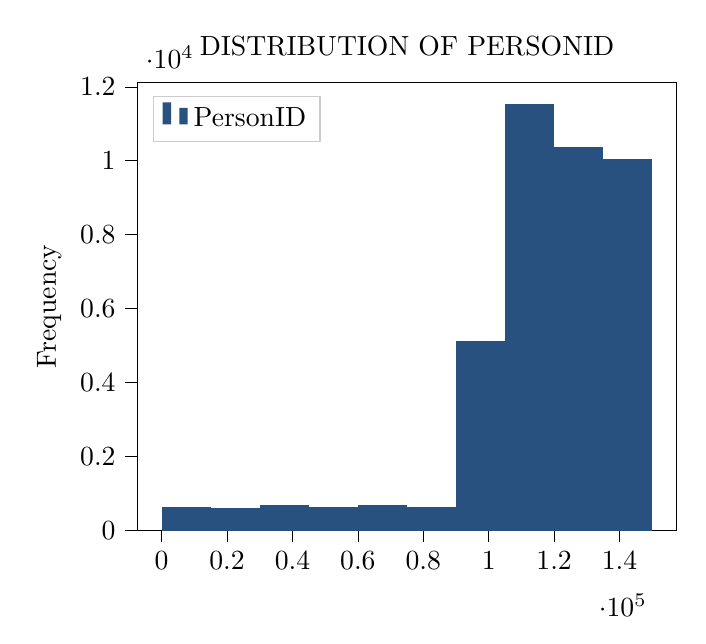
\begin{tikzpicture}

\definecolor{color0}{rgb}{0.156862745098039,0.317647058823529,0.501960784313725}

\begin{axis}[
legend cell align={left},
legend style={at={(0.03,0.97)}, anchor=north west, draw=white!80.0!black},
tick align=outside,
tick pos=left,
title={\printsubsection{\MakeUppercase{Distribution of PersonID}}},
x grid style={white!69.01960784313725!black},
xmin=-7476.85, xmax=157497.85,
xtick style={color=black},
y grid style={white!69.01960784313725!black},
ylabel={Frequency},
ymin=0, ymax=12125.4,
ytick style={color=black}
]
\draw[fill=color0,draw opacity=0] (axis cs:22,0) rectangle (axis cs:15019.7,640);
\addlegendimage{ybar,ybar legend,fill=color0,draw opacity=0};
\addlegendentry{PersonID}

\draw[fill=color0,draw opacity=0] (axis cs:15019.7,0) rectangle (axis cs:30017.4,614);
\draw[fill=color0,draw opacity=0] (axis cs:30017.4,0) rectangle (axis cs:45015.1,691);
\draw[fill=color0,draw opacity=0] (axis cs:45015.1,0) rectangle (axis cs:60012.8,638);
\draw[fill=color0,draw opacity=0] (axis cs:60012.8,0) rectangle (axis cs:75010.5,703);
\draw[fill=color0,draw opacity=0] (axis cs:75010.5,0) rectangle (axis cs:90008.2,632);
\draw[fill=color0,draw opacity=0] (axis cs:90008.2,0) rectangle (axis cs:105005.9,5122);
\draw[fill=color0,draw opacity=0] (axis cs:105005.9,0) rectangle (axis cs:120003.6,11548);
\draw[fill=color0,draw opacity=0] (axis cs:120003.6,0) rectangle (axis cs:135001.3,10370);
\draw[fill=color0,draw opacity=0] (axis cs:135001.3,0) rectangle (axis cs:149999,10058);
\end{axis}

\end{tikzpicture}